\section{Zusammenfassung und Diskussion}

In Versuch 234 beschäftigen wir uns mit der Untersuchung der Spektren verschiedener Lichtquellen. Hier unterscheiden wir zwischen Temperaturstrahlern und Nichttemperaturstrahlern. Temperaturstrahler, wie beispielsweise eine Glühlampe, basieren auf dem Phänomen, dass jeder Körper, dessen Temperatur größer als $0\si{\kelvin}$ ist, elektromagnetische Strahlung abstrahlt, deren Intensitätsverteilung abhängig von der Wellenlänge dem Planck'schen Strahlungsgesetz folgt. Bei den Nichttemperaturstrahlern ist die Erzeugung von Licht entweder auf Anregung von Atomzuständen, zum Beispiel bei einer Natriumdampflampe, oder der Rekombination von Elektron-Loch-Paaren in Halbleitern, also LEDs, zurückzuführen.

Im ersten Versuchsteil untersuchten wir das Spektrum des wohl bekanntesten Temperaturstrahlers, der Sonne. Mit einem Gitterspektroskop nahmen wir das Spektrum des Tageslichts einmal direkt und einmal durch ein Fenster auf. Wir konnten beobachten, dass es sich um ein kontinuierliches Spektrum handelt, wie es von Temperaturstrahlern zu erwarten ist. 

\begin{figure}[H]
  \centering
  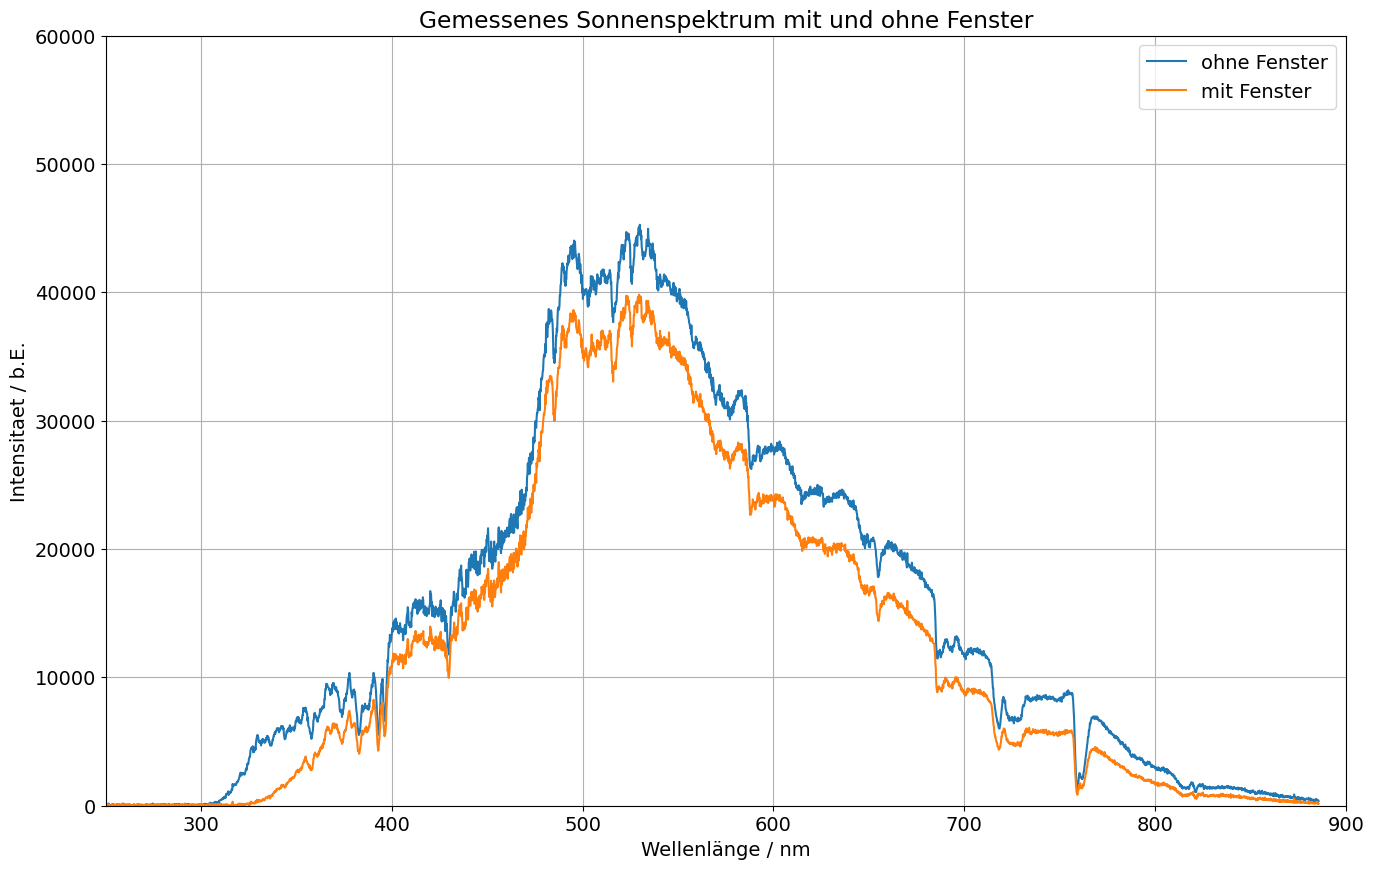
\includegraphics[width=.9\textwidth]{files/plots/himmel_m_o_g.png}
  \caption{Spektrum des Tageslichts mit und ohne Fenster.}
  \label{fig:himmel_m_o_g_zsmf}
\end{figure}


Im Vergleich des Spektrums durch das Fenster mit dem, das direkt aufgezeichnet wurde, konnten wir beobachten, dass durch die Scheibe über den gesamten Wellenlängenbereich hinweg die Intensität des Lichts durch die Absorption der Glasscheibe abgeschwächt wird. Bei genauerer Betrachtung der Absorption konnten wir sehen, dass diese im Bereich von Wellenlängen unter $400\si{\nano\meter}$, also im nicht-sichtbaren UV-Bereich, am höchsten und im Bereich des sichtbaren Lichts am niedrigsten ist.

Die vielen im Spektrum deutlich sichtbaren lokalen Minima sind durch die Absorption von Licht bestimmter Wellenlängen in den Atmosphärenschichten der Sonne und der Erde zu erklären. Diese Absorptionslinien, genannt \glqq{}Fraunhoferlinien\grqq{} sind speziellen Wellenlängen zugeordnet, welche wir mit den Positionen der Linien in unsren aufgezeichneten Spektrum verglichen. Die Werte sind, mit der jeweiligen Abweichung vom Literaturwert in \tabref{tab:fraunhofer_vergleich_zsmf} zusammengefasst. Als Fehler für die beobachteten Wellenlängen sind wir jeweils von $\pm 1\si{\nano\meter}$ ausgegangen.

\begin{table}[h]
  \centering
  \caption{Vergleich der erwarteten und gemessenen Wellenlängen der Fraunhofer- und Balmerlinien}
  \vspace*{0.5em}
  \begin{tabular}{c|c|c|c}
      \hline
      Linie & Literaturwert [nm] & Abgelesener Wert [nm] & Abweichung [$\sigma$] \\
      \hline
      K  & 393.4 & 393.0 & 0.4 \\
      H  & 396.8 & 396.1 & 0.7 \\
      G  & 430.8 & 429.8 & 1.0 \\
      F  & 486.1 & 485.2 & 0.91 \\
      b1 & 518.4 & 516.7 & 1.7 \\
      E  & 527.0 & 526.2 & 0.8 \\
      D3 & 587.6 & 588.4 & 0.8 \\
      D2 & 589.0 & 589.0 & 0.0 \\
      D1 & 589.6 & 589.7 & 0.11 \\
      C  & 656.3 & 655.0 & 1.3 \\
      B  & 686.7 & 686.7 & 0.0 \\
      A  & 759.4 & 759.4 & 0.0 \\
      \hline\hline
      $\mathrm{H}_{\alpha}$ & 656.3 & 655.0 & 1.3\\
      $\mathrm{H}_{\beta}$ & 486.1 & 485.2 & 0.91\\
      $\mathrm{H}_{\gamma}$ & 434.0 & 433.4 & 0.61\\
      $\mathrm{H}_{\delta}$ & 410.1 & 409.5 & 0.61\\
      \hline
  \end{tabular}
  \label{tab:fraunhofer_vergleich_zsmf}
\end{table}

Unter anderem als lokale Minima im Sonnenlichtspektrum zu beobachten sind die Linien der Balmerserie, welche auf Anregungen in Wasserstoffatom zurückzuführen sind. Die beobachteten Positionen der $H_{\alpha}-, H_{\beta}-, H_{\gamma}-, H_{\delta}-$Linien der Balmerserie verglichen wir ebenfalls mit den Literaturwerten, zusammengefasst in derselben Tabelle.

Insgesamt ist die Abweichung der beobachteten Absorptionslinien von den Literaturwerten sehr gering. Die dennoch sichtbaren Unterschieden sind vermutlich zu Großteilen auf das wolkige Wetter am Versuchstag, sowie Störungen und Reflexionen durch die umliegenden Gebäude zurückzuführen.

Im darauf folgenden Versuchsteil betrachteten wir qualitativ die Spektren verschiedener Lichtquellen. Hierunter untersuchten wir das Licht verschiedenfarbiger LEDs, eines Lasers und einer Energiesparlampe als Beispiele für Nichttemperaturstrahler, sowie das einer Glühlampe als ein klassisches Beispiel für einen Temperaturstrahler. Wie in der Theorie beschrieben, konnten wir beobachten, dass die LEDs, der Laser und die Energiesparlampe diskrete Spektren aufweisen. Dabei basiert die Erzeugung von weißem Licht bei den weißen LEDs und der Energiesparlampe auf verschiedenen Methoden. Die Glühlampe wies ein kontinuierliches Spektrum auf, von welchem große Teile außerhalb des sichtbaren Wellenlängenbereichs lagen. Dies zeigte auch, dass diese im Vergleich zu den anderen Lichtquellen viel weniger energieeffizient ist.

Im abschließenden großen Versuchsblock setzen wir uns mit dem Spektrum einer Natriumdampflampe auseinander. Als Beispiel für eine Gasentladungslampe weist diese ein diskretes Spektrum auf, welches durch eine Vielzahl an Spektrallinien über den gesamten beobachteten Wellenlängen charakterisiert ist. Wir betrachteten zunächst das Spektrum in einem Wellenlängenbereich von $350$ bis $550\si{\nano\meter}$. Hier sind Spektrallinien mit geringer Intensität zu beobachten. Wir notierten die Wellenlängen aller gut sichtbarer Linien für den späteren Vergleich. Im Bereich zwischen $590$ und $600\si{\nano\meter}$ befindet sich im Natriumspektrum die markante D-Linie. Auch die Wellenlänge dieser Linie selbst, sowie die Wellenlängen einiger umliegender Linien notierten wir uns. Zuletzt zeichneten wir noch die Wellenlängen einiger markanter Linien im oberen Wellenlängenbereich von $650$ bis $850\si{\nano\meter}$ auf.

Zum Vergleich der beobachteten mit den theoretisch vorhersagten Positionen der Spektrallinien betrachteten wir dann die Übergänge $md \to 3p$ der 1. Nebenserie, die Übergänge $ms \to 3p$ der 2. Nebenserie, sowie die $mp \to 3s$ der Hauptserie. Die Energie $E_{3p}$, welche wir für die Berechnungen der Wellenlängen der Übergänge zum $3p$-Zustand benötigen, bestimmten wir auf einen Wert von
\begin{align}
  E_{3p} = -3.0279 \pm 0.0019\si{\electronvolt}.
\end{align}

Mit diesem bestimmten wir anhand der Formel $\lambda_m \approx \flatfrac{hc}{\qty(\frac{E_{Ry}}{m^2} - E_{3p})}$ für die Quantenzahlen $m=3,\dots,12$ die erwarteten Wellenlängen der Spektrallinien. Diese sind in \tabref{tab:wellenlaengen_1ns_zsmf} zusammen mit den von uns beobachteten Wellenlängen, welche wir diesen zuordnen konnten, aufgelistet.

\begin{table}[H]
  \centering
  \caption{Vergleich der berechneten und gemessenen Wellenlängen der 1. Nebenserie $md \to 3p$.}
  \vspace*{0.5em}
  \begin{tabular}{c c c c}
      \hline
      $m$ & $\lambda_{\text{theo.}}$ [nm] & $\lambda_{\text{beob.}}$ [nm] & Abweichung \\
      \hline
      3  & $817.7 \pm 1.000$ & $817.7 \pm 1$ & 0.01$\sigma$ \\
      4  & $569.4 \pm 0.5$ & $567.1 \pm 1$ & 2.03$\sigma$ \\
      5  & $499.2 \pm 0.4$ & $496.9 \pm 2$ & 1.13$\sigma$ \\
      6  & $467.9 \pm 0.4$ & $469.2 \pm 1$ & 1.28$\sigma$ \\
      7  & $450.8 \pm 0.4$ & $450.0 \pm 1$ & 0.77$\sigma$ \\
      8  & $440.4 \pm 0.3$ & $438.1 \pm 1$ & 2.20$\sigma$ \\
      9  & $433.5 \pm 0.3$ & $432.6 \pm 1$ & 0.88$\sigma$ \\
      10 & $428.7 \pm 0.3$ & $429.2 \pm 1$ & 0.46$\sigma$ \\
      11 & $425.3 \pm 0.3$ & $426.0 \pm 1$ & 0.72$\sigma$ \\
      12 & $422.7 \pm 0.3$ & $423.1 \pm 1$ & 0.44$\sigma$ \\
      \hline
  \end{tabular}
  \label{tab:wellenlaengen_1ns_zsmf}
\end{table}

Wir können sehen, dass die Abweichung bei den meisten Linien unter einem $\sigma$ liegt. Bei den Vergleichen mit einer signifikanteren Abweichung kann es durchaus sein, dass den theoretisch vorhersagten Linien falsche beobachtete Linien zugeordnet wurden.